% Original book p12; original base PDF p16; input PDF p19; p012_s01 四、3
% Role: answer; original field: diagrams[1].tikz
% Compile with XeLaTeX from this figures/ directory.
\documentclass[12pt,tikz,border=5pt]{standalone}
\usepackage{fontspec}
\setmainfont[Path=../fonts/]{DroidSansFallback.ttf}
\setsansfont[Path=../fonts/]{DroidSansFallback.ttf}
\usepackage{amsmath,amssymb}
\usepackage{tikz}
\usetikzlibrary{calc,angles,quotes,arrows.meta,decorations.pathreplacing,decorations.pathmorphing,decorations.markings,patterns,positioning,fit,backgrounds,matrix,intersections,shapes.geometric}
\begin{document}
\color{black}
\tikzset{every picture/.append style={color=black}}
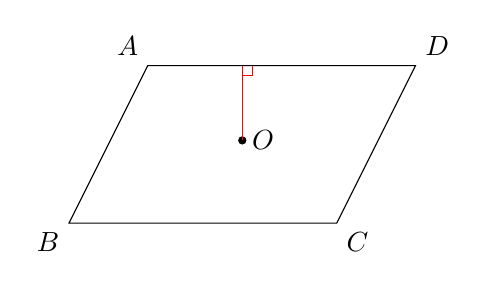
\begin{tikzpicture}\coordinate(B)at(0,0);\coordinate(A)at(1,2);\coordinate(D)at(4.4,2);\coordinate(C)at(3.4,0);\draw(A)--(B)--(C)--(D)--cycle;\foreach \p/\pos in {A/above left,B/below left,C/below right,D/above right}{\node[\pos]at(\p){$\p$};}\fill(2.2,1.05)circle(1.5pt)node[right]{$O$};\draw[red](2.200000,1.050000)--(2.200000,2.000000);\draw[red](2.330000,2.000000)--(2.330000,1.870000)--(2.200000,1.870000);\end{tikzpicture}

\end{document}
